\documentclass{ExamJHSMath}
\showAnswer{1}


\begin{document}

\chapter[八年级下学期期中试卷数学]{
  \hspace*{-0.3em}
  \headLine{2023年}{九年级上学期期末试卷}{数学}{}
}


\subsection{\Choices{12}{3}}
\begin{enumerate}[ref={\arabic*}]

\item 下列图形从中任取一个是中心对称图形的概率是 \choice{}
\begin{center}
\vspace{-2ex}
  \includegraphics[height=1.2cm]{figure1.png}
\vspace{-2ex}
\end{center}
\options
  {$\dfrac{1}{4}$}
  {$\dfrac{1}{2}$}
  {$\dfrac{3}{4}$}
  {$1$}

\item 下列事件是随机事件的是 \choice{}
\options
  {明天太阳从东方升起}
  {任意画一个三角形,其内角和是 $360^\circ$}
  {通常温度降到 0 ℃以下,纯净的水结冰}
  {射击运动员射击一次,命中靶心}

\item 重复试验:抛掷同一枚啤酒瓶盖 1000 次,经过统计得“凹面向上”的频率约为 0.53.则可以估计抛掷这枚啤酒瓶盖出现“凸面向上”的概率约为 \choice{}
\options
  {0.53}
  {0.51}
  {0.50}
  {0.47}

\item 若实数 $x, y$ 满足 $(x+y)(x+y-1)=2$,则 $x+y=$ \choice{}
\options
  {$-1$}
  {2}
  {$-1$ 或 2}
  {1 或 $-2$}

\item 抛物线 $y=3(x-2)^{2}+5$ 的顶点坐标是 \choice{}
\options
  {$(2,5)$}
  {$(-2,-5)$}
  {$(-2,5)$}
  {$(2,-5)$}

\item 如图 $\angle DCE$ 是 $\odot O$ 内接四边形 $ABCD$ 的个外角, 若 $\angle DCE=82^\circ$, 那么 $\angle BOD$ 的度数为 \choice{}
\options
  {$160^\circ$}
  {$162^\circ$}
  {$164^\circ$}
  {$170^\circ$}

  \begin{figure}[htp] \centering
    \vspace{-2ex}
    \begin{minipage}[t]{.32\textwidth} \centering
      \begin{tikzpicture}[scale=.45, every node/.style={scale=.8}]
        \tkzDefPoints{0/0/O,1/-1.5/C}
        \tkzDefPointBy[rotation= center O angle 60](C) \tkzGetPoint{D}
        \tkzDefPointBy[rotation= center O angle 160](C) \tkzGetPoint{A}
        \tkzDefPointBy[rotation= center C angle -82](D) \tkzGetPoint{E0}
        \tkzDefBarycentricPoint(C=1,E0=1) \tkzGetPoint{E}
        \tkzDrawCircle(O,C)
        \tkzInterLC(C,E)(O,C) \tkzGetPoints{X}{B}
        \tkzDrawSegments(B,C C,D A,D A,B C,E)
        \tkzDrawPoints(O)
        \tkzLabelPoints[above](A)
        \tkzLabelPoints[below](C,E,O)
        \tkzLabelPoints[left](B)
        \tkzLabelPoints[right](D)
      \end{tikzpicture}
      \caption*{题6图}
    \end{minipage}
    \begin{minipage}[t]{.32\textwidth} \centering
      \begin{tikzpicture}[scale=.6, every node/.style={scale=.8}]
        \tkzDefPoints{0/0/O,1/1/R0,-2/3/A}
        \tkzDrawCircle[R](O,1.5cm)        \tkzDefPointOnCircle[angle=0,center=O,radius=1.5cm] \tkzGetPoint{C}
        \tkzDefBarycentricPoint(C=3,O=2) \tkzGetPoint{M}
        \tkzDefShiftPoint[M](0,1){M0}
        \tkzInterLC(M,M0)(O,C) \tkzGetPoints{A}{B}
        \tkzInterLC(O,M)(O,C) \tkzGetPoints{D}{D0}
        \tkzDrawSegments[color=black](A,B C,D O,A)
        \tkzMarkRightAngle[size=0.2](A,M,C)
        \tkzDrawPoints(O,C,M)
        \tkzLabelPoints[above](A)
        \tkzLabelPoints[below](O,B)
        \tkzLabelPoints[left](D)
        \tkzLabelPoints[right](C)
        \tkzLabelPoints[above left](M)
      \end{tikzpicture}
      \caption*{题8图}
    \end{minipage}
    \begin{minipage}[t]{.32\textwidth} \centering
      \begin{tikzpicture}[scale=.42, every node/.style={scale=.8}]
        \tkzDefPoints{0/0/O,1/1/R0,-2/3/A}
        \tkzDrawCircle[R](O,1.5cm)
        \tkzDefTangent[from with R=A](O,1.5cm) \tkzGetPoints{P}{C}
        \tkzDefPointOnCircle[angle=-100,center=O,radius=1.5cm] \tkzGetPoint{D}
        \tkzDefTangent[at=D](O) \tkzGetPoint{D0}
        \tkzInterLL(D,D0)(A,P) \tkzGetPoint{B}
        \tkzDrawSegments[color=black](A,P A,C P,B B,D)  
        \tkzDrawPoints(O)
        \tkzLabelPoints[above](A,C)
        \tkzLabelPoints[below](O,B,D)
        \tkzLabelPoints[above left](P)
      \end{tikzpicture}
      \caption*{题9图}
    \end{minipage}
    \vspace{-3ex}
  \end{figure}

\item 函数 $y=ax-a$ 和 $y=ax^{2}+2$ ($a$ 为常数,且 $a\neq 0$),在同平面直角坐标系中的大致图象可能是 \choice{}
\options
  {
\begin{tikzpicture}[scale=.7, every node/.style={scale=.8}]
    \tkzInit[xmin=-1,xmax=1,ymin=-1,ymax=1]
    \tkzDrawXY[noticks,>=latex]
    \tkzDefPoint(0,0){O}
    \tkzLabelPoints[below right](O)
    \draw[domain=-1:1,samples=80,thick] plot(\x,{1.8*(\x)^2-0.5});
    \draw[domain=-0.8:1.2,samples=80,thick] plot(\x,{\x+0.4});
  \end{tikzpicture}}
  {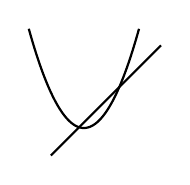
\begin{tikzpicture}[scale=.7, every node/.style={scale=.8}]
    \tkzInit[xmin=-1,xmax=1,ymin=-1,ymax=1]
    \tkzDrawXY[noticks,>=latex]
    \tkzDefPoint(0,0){O}
    \tkzLabelPoints[above left](O)
    \draw[domain=-1:1,samples=80,thick] plot(\x,{1.8*(\x)^2-0.5});
    \draw[domain=-0.6:1.4,samples=80,thick] plot(\x,{\x-0.4});
  \end{tikzpicture}}
  {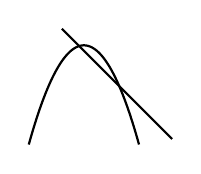
\begin{tikzpicture}[scale=.7, every node/.style={scale=.8}]
    \tkzInit[xmin=-1,xmax=1,ymin=-1,ymax=1]
    \tkzDrawXY[noticks,>=latex]
    \tkzDefPoint(0,0){O}
    \tkzLabelPoints[below left](O)
    \draw[domain=-1:1,samples=80,thick] plot(\x,{-1.8*(\x)^2+0.5});
    \draw[domain=-0.4:1.6,samples=80,thick] plot(\x,{-\x+0.4});
  \end{tikzpicture}}
  {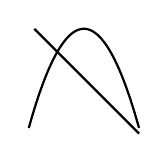
\begin{tikzpicture}[scale=.7, every node/.style={scale=.8}]
    \tkzInit[xmin=-1,xmax=1,ymin=-1,ymax=1]
    \tkzDrawXY[noticks,>=latex]
    \tkzDefPoint(0,0){O}
    \tkzLabelPoints[below left](O)
    \draw[domain=-1:1,samples=80,thick] plot(\x,{-1.8*(\x)^2+0.5});
    \draw[domain=-0.9:1,samples=80,thick] plot(\x,{-\x-0.4});
  \end{tikzpicture}}

\item 如图,$\odot O$ 的直径 $CD=30$,$AB$ 是 $\odot O$ 的弦,$AB\perp CD$.垂足为$M$,$OM:OC=3:5$,则 $AB$ 的长为 \choice{}
\options
  {8}
  {24}
  {16}
  {$2\sqrt{91}$}

\item 如图,$AB$、$AC$、$BD$是 $\odot O$ 的切线,切点分别为 $P$、$C$、$D$.若 $AB=4$,$MC=3$,则 $BD$ 的长是 \choice{}
\options
  {1}
  {2}
  {3}
  {4}

\item 某超市一月份的营业额为 200 万元,一、二、三月份的总营业额为 1000 万元,设平均每月营业额的增长率为 $x$,则由题意列方程为 \choice{}
\options
  {$200+200\times 2x=1000$}
  {$200(1+x)^{2}=1000$}
  {$200+200\times 3x=1000$}
  {$200 \left[ 1+(1+x)+(1+x)^{2} \right]=1000$}

\item 下列结论不正确的是 \choice{}
\options
  {所有的矩形都相似}
  {所有的正三角形都相似}
  {所有的等腰直角三角形都相似}
  {所有的正八边形都相似}

\item 已知二次函数 $y=ax^{2}+bx+c$ 的图象如图所示,下列结论:① $abc>0$;② $2a-b<0$;③ $4a-2b+c<0$;④ $(a+c)^{2}<b^{2}$,其中正确的个数是 \choice{}
\options
  {1}
  {2}
  {3}
  {4}

\end{enumerate}

  \begin{figure}[htp] \centering
    \vspace{-2ex}
    \begin{minipage}[t]{.32\textwidth} \centering
      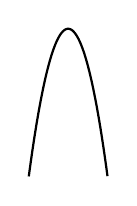
\begin{tikzpicture}[scale=.4, every node/.style={scale=.8}]
        \tkzInit[xmin=-2.4,xmax=1.8,ymin=-1,ymax=3]
        \tkzAxeX
        \tkzDrawY[noticks,>=latex]
        \tkzDefPoint(0,0){O}
        \draw[domain=-2:0.5,samples=80,thick] plot(\x,{-3*(\x)^2-4.5*\x+1.2});
      \end{tikzpicture}
      \caption*{题12图}
    \end{minipage}
    \begin{minipage}[t]{.32\textwidth} \centering
      \begin{tikzpicture}[scale=.55, every node/.style={scale=.8}]
        \tkzDefPoints{0/0/O,3/0.7/A,4/0/B}
        \tkzDefPointBy[rotation=center O angle 40](A) \tkzGetPoint{C}
        \tkzDefPointBy[rotation=center O angle 40](B) \tkzGetPoint{D}
        \tkzDrawSegments(O,A O,B A,B O,C O,D C,D)
        \tkzDrawArc[color=black,style=dashed](O,A)(C)
        \tkzDrawArc[color=black,style=dashed](O,B)(D)
        \tkzLabelPoints[above](C,D)
        \tkzLabelPoints[above right](A)
        \tkzLabelPoints[below left](O)
        \tkzLabelPoints[below right](B)
      \end{tikzpicture}
      \caption*{题14图}
    \end{minipage}
    \begin{minipage}[t]{.32\textwidth} \centering
      \begin{tikzpicture}[scale=.35, every node/.style={scale=.8}]
        \tkzInit[xmin=-1,xmax=7,ymin=-1,ymax=2]
        \tkzDrawXY[noticks,>=latex]
        \tkzDefPoints{4/2/P,2/0/A,6/0/B,0/0/O}
        \tkzDrawArc[delta=20,thick,color=black](P,A)(B)
        \tkzDrawPoints(P)
        \tkzLabelPoints[below](A,B,P)
      \end{tikzpicture}
      \caption*{题20图}
    \end{minipage}
    \vspace{-3ex}
  \end{figure}


\subsection{\Completions{8}{3}}
\begin{enumerate}[resume,ref={\arabic*}]

  \item 抛物线 $y=2x^{2}+1$ 向左平移 1 个单位,再向下平移 2 个单位,所得到的抛物线是 \\ \blank[4]{}。
  
  \item 如图,将 $\triangle AOB$ 绕点 $O$ 按逆时针方向旋转 $40^\circ$ 后得到 $\triangle COD$,若 $\angle AOB=10^\circ$,则 $\angle AOD$ 的角度是 \blank{}。
  
  \item 若关于 $x$ 的一元二次方程 $(m-1)x^{2}+x+m^{2}-1=0$ 有一个根为 0,则 $m=$ \blank{}。
  
  \item 点 $M(1,2)$ 关于原点对称的点的坐标是 \blank{}。
  
  \item 圆锥的底面半径为 5,高为 12,则该圆锥的侧面积为 \blank{}。
  
  \item 有 5 张看上去无差别的卡片,正面分别写着1,2,3,4,5,洗匀后正面向下放在桌子上,从中随机抽取 2 张,抽出的卡片上的数字恰好是两个连续整数的概率是 \blank{}。
  
  \item 两个相似三角形一组对应角平分线的长分别是 $\rm{2\ cm}$ 和 $\rm{5\ cm}$,在这两个是三角形的一组对应中线中,如果较短的中线是 $\rm{3\ cm}$,那么较长的中线的长为 \blank{}。
  
  \item 如图,以点 $P$ 为圆心的圆弧与 $x$ 轴交于 $A$,$B$ 两点,点 $P$ 的坐标为 $(4,-2)$,点 $A$ 的坐标为 $(2,0)$,则点 $B$ 的坐标为 \blank{}。
\end{enumerate}



\subsection{\Explanations{6}{60}}
\begin{enumerate}[resume,ref={\arabic*}]

  \item \scores{6} 解下列方程
  \begin{tasks}[](2)
    \task $x^{2}-2x-8=0$
    \task $(x-1)^{2}=2x(x-1)$
    \vspace{6ex}
  \end{tasks}

  \item \scores{10} 初三年级“黄金分割项目活动”展示,为了解全体初三年级同学的活动成绩,抽取了部分参加活动的同学的成绩进行统计后,分为“优秀”,“良好”,“一般”,“较差”四个等级,并根据成绩绘制成如图两幅不完整的统计图,请结合统计图中的信息,回答下列问题:
  \sidefig{R}{
    \vspace{-2ex}
    \begin{minipage}[t]{.24\textwidth} \centering
      \begin{tikzpicture}[xscale=.36,yscale=.55, every node/.style={scale=.8},>=Stealth,font=\Kai]
        \draw (0,0) node[below left]{$O$};
        \draw[->](0,0)--(0,5.5) node[right]{人数};  
        \draw[dashed]
          (0.1,1)--(0,1) node[left]{$10$}
          (0.1,2)--(0,2) node[left]{$20$}
          (0.1,3)--(0,3) node[left]{$30$}
          (0.1,4)--(0,4) node[left]{$40$}
          (0.1,5)--(0,5) node[left]{$50$};  
        \draw[->](0,0)--(8,0) node[below right]{等级};
        \foreach \x/\xtext in{2/优秀,4/良好,6/一般,8/较差}
          \node[below]at(\x-1,0){\xtext};  
        \draw[fill=gray!40]
          (0.5,0)--(0.5,2.4)--(1.5,2.4)--(1.5,0)
          (4.5,0)--(4.5,3.0)--(5.5,3.0)--(5.5,0)
          (6.5,0)--(6.5,1.8)--(7.5,1.8)--(7.5,0);  
        \draw[dashed]
          (0,2.4)--(1.0,2.4) node[above]{$24$}
          (0,3.0)--(5.0,3.0) node[above]{$30$}
          (0,1.8)--(7.0,1.8) node[above]{$18$};
      \end{tikzpicture}  
    \end{minipage}
    \begin{minipage}[t]{.2\textwidth} \centering
      \begin{tikzpicture}[scale=.6, every node/.style={scale=.8},>=Stealth]
        \tkzDefPoints{0/0/O,1.2/0/A,-1.5/0.2/D}
        \tkzDrawSector[R](O, 2cm)(0,90)
        \tkzDrawSector[R](O, 2cm)(90,144)
        \tkzDrawSector[R](O, 2cm)(144,216)
        \tkzDrawSector[R](O, 2cm)(216,360)
        \tkzDefPointBy[rotation=center O angle 45](A) \tkzGetPoint{B}
        \tkzLabelPoint[above](B){一般}
        \tkzLabelPoint[below](B){25\%}
        \tkzDefPointBy[rotation=center O angle 117](A) \tkzGetPoint{C}
        \tkzLabelPoint[above](C){较差}
        \tkzLabelPoint[below](C){15\%}
        \tkzLabelPoint(D){优秀}
        \tkzDefPointBy[rotation=center O angle 288](A) \tkzGetPoint{E}
        \tkzLabelPoint[above](E){良好}
        \tkzLabelPoint[below](E){40\%}
      \end{tikzpicture}
    \end{minipage}
    \vspace{-2ex}
  }
  \begin{enumerate}
    \item 扇形统计图中“优秀”所对应扇形的圆心角为 \blank{} 度,并将条形统计图补充完整;
    \item 如果学校初三年级共有 340 名学生,则参加“黄金分割项目活动”比赛成绩良好的学生有 \blank{} 人;
    \item 此次活动中有四名同学获得满分,分别是甲,乙,丙,丁,现从这四名同学中挑选两名同学参加校外举行的“黄金分割项目活动”展示,请用列表法或画树状图法,求出选中的两名同学恰好是甲、丁的概率。
  \end{enumerate}
  \vspace{10ex}

  \item \scores{10} 如图,$AB$为 $\odot O$ 的直径,$C$、$F$ 为 $\odot O$ 上两点,且点 $C$ 为弧 $BF$ 的中点,过点 $C$ 作 $AF$ 的垂线,交 $AF$ 的延长线于点 $E$,交 $AB$ 的延长线于点 $D$。
  \sidefig{R}{
    \begin{tikzpicture}[scale=.7, every node/.style={scale=.8}]
      \tkzDefPoints{0/0/O, 1/-1.5/E0}
      \tkzDrawCircle[R](O,1.5cm)
      \tkzDefPointOnCircle[angle=36,center=O,radius=1.5cm] \tkzGetPoint{A}
      \tkzDefPointOnCircle[angle=-90,center=O,radius=1.5cm] \tkzGetPoint{C}
      \tkzDefPointsBy[projection=onto C--E0](A){E}
      \tkzInterLC(A,O)(O,A) \tkzGetPoints{A}{B}
      \tkzInterLC(A,E)(O,A) \tkzGetPoints{A}{F}
      \tkzInterLL(A,B)(C,E) \tkzGetPoint{D}
      \tkzDrawSegments[color=black](A,E C,E A,D D,E A,C)
      \tkzMarkRightAngle[size=0.15](A,E,C)
      \tkzDrawPoints(O)
      \tkzLabelPoints[above](O,A)
      \tkzLabelPoints[below](C,D,E)
      \tkzLabelPoints[left](B)
      \tkzLabelPoints[right](F)
    \end{tikzpicture}
  }
  \begin{enumerate}
    \item 求证:$DE$ 是 $\odot O$ 的切线;
    \item 若 $AE=3$,$DE=4$,求 $\odot O$ 的半径的长。
  \end{enumerate}
  \vspace{20ex}
  
  \sidefig{R}{
    \begin{tikzpicture}[scale=.8, every node/.style={scale=.8}]
      \tkzDefPoints{0/0/B,2/0/C,2.8/1.5/D,0.8/0/E,2.4/0.8/M}
      \tkzDefParallelogram(B,C,D) \tkzGetPoint{A}
      \tkzDrawPolygon(A,B,C,D)
      \tkzInterLL(D,E)(A,M) \tkzGetPoint{F}
      \tkzDrawSegments(A,E E,D A,F)
      \tkzMarkRightAngle[size=0.15](A,E,B)
      \tkzLabelPoints[above](A,D)
      \tkzLabelPoints[below](B,C,E,F)
    \end{tikzpicture}
  }
  \item \scores{12} 如图,在平行四边形 $ABCD$ 中,过点 $A$ 作 $AE\perp BC$,垂足为 $E$,连接 $DE$,$F$ 为线段 $DE$ 上一点,且 $\angle AFE=\angle B$。
  \begin{enumerate}
    \item 求证: $\angle DFA=\angle ECD$;
    \item $\triangle ADF$ 与 $\triangle DEC$ 相似吗?为什么?
    \newpage
    \item 若 $AB= 4$,$AD= 3\sqrt{3}$,$AE=3$,求 $AF$ 的长。
  \end{enumerate}
  \vspace{15ex}
  
  \item \scores{12} 某汽车 4S 店销售 A,B 两种型号的轿车,具体信息如下表:
  \begin{table}[htbp] \centering
    \renewcommand\arraystretch{1.2}{
      \begin{tabular}{|c|c|c|c|}
      \hline
      & 每辆进价(万元) & 每辆售价(万元) & 每季度销量(辆) \\ \hline
        A & 60 & $x$ & $-x+100$ \\ \hline
        B & 50 & $y$ & $-2y+150$ \\ \hline
      \end{tabular}
    }
    \caption*{(注:厂家要求 4S 店每季度 B 型轿车的销量是A型轿车销量的2倍)}
  \end{table}
  \vspace{-2ex}
  根据以上信息解答下列问题:
  \begin{enumerate}
    \item 用含 $x$ 的代数式表示 $y$;
    \item 今年第三季度该 4S 店销售 A,B 两种型号:轿车的利润恰好相同(利润不为0),试求 $x$ 的值;
    \item 求该 4S 店第四季度销售这两种轿车能获得的最大利润。
  \end{enumerate}
  \vspace{20ex}

  \item \scores{10} 如图,已如抛物线 $y=ax^{2}+bx+c, \ (a\neq 0)$ 与 $x$ 轴交于点 $A(1,0)$ 和点 $B(-3,0)$,与 $y$ 轴交于点 $C$,且 $OC=OB$。
  \sidefig{R}{
    \begin{tikzpicture}[scale=.4, every node/.style={scale=.8}]
      \tkzInit[xmin=-5,xmax=2,ymin=-2,ymax=4]
      \tkzDrawXY[noticks,>=latex]
      \tkzDefPoint(0,0){O} \tkzDefPoint(-1,4.5){P1} \tkzDefPoint(-1,-2.5){P2}
      \tkzDefPoint(1,0){A} \tkzDefPoint(-3,0){B} \tkzDefPoint(0,3){C} \tkzDefPoint(-1.5,3.75){E}
      \draw[domain=-3.5:1.5,samples=80,thick] plot(\x,{-(\x)^2-2*\x+3});
      \tkzDrawSegment[style=dashed,color=black](P1,P2)
      \tkzDrawPoints[color=black](A,B,C,E)
      \tkzLabelPoints[left](C)
      \tkzLabelPoints[below right](O)
      \tkzLabelPoints[above left](B,E)
      \tkzLabelPoints[above right](A)
    \end{tikzpicture}
  }
  \begin{enumerate}
    \item 求点 $C$ 的坐标和此抛物线的解析式;
    \item 若点 $E$ 为第二象限抛物线上一动点,连接 $BE$,$CE$,$BC$,求 $\triangle BCE$ 面积的最大值。
  \end{enumerate}
  \vspace{10ex}

\end{enumerate}


\end{document}
